\chapter{Approach to estimate vehicle motion}

\section{Objectives}
\subsection{Primary objectives}
The goal is to build a software system, using computer vision algorithms. First of all, it should be able to estimate the frame-to-frame motion of a racing car and the momentary orientation of the camera with respect to the ground plane. Secondly, at any time, the system should be able to create a birds eye view map of the environment that is in front of the car, in particular the positions of the cones which are used to mark the drivable path.\bigskip 

\subsection{Secondary objectives}
When a good solution is found to these two problems, the system could be expanded and obstacles, side barriers etc. could be entered into the map previously mentioned. Based on the previous features of the system, two additional features could be added: reconstruction of the car's trajectory over time and building a global map from the instantaneous map.\bigskip

These last two additional features are a nice addition to the primal goals, but will only be investigated once the primal goals are working properly.

\section{Sequencer}
First, we need a way to step through the footage of the race car efficiently. For this purpose, a sequencer is built, this sequencer takes footage from a camera mounted to a racing car. The footage from the camera is a video, to process this, each frame of the video is stored as a separate image. These images can be fed to the sequencer to process them. The sequencer takes 1 of these images at a time as input and stores it in a buffer. This image is converted into a grayscale image and cropped so the horizon is (as much as possible) out of the image. This converted image is then inserted into a FIFO of length N (right now, N is set at two). The two images in the FIFO are now ready for processing, the specifics of this processing will be discussed later. The visualisation component takes the images in the FIFO to visualise everything (keypoints, motion vectors...).\bigskip

With specific keys, it is possible to go forwards and backwards through the sequence. When advancing through the sequence a new image is loaded in the buffer. It is also possible to jump multiple frames ahead/backwards. The buffer is then cleared and filled with the correct images. With a press of the space bar, the sequencer continuously takes the next input image and loops the sequence.\bigskip

Figure \autoref{fig:scheme} shows an overview of the different steps the sequencer goes through. The "Process Image Pair" component calculates the Homography \underline{${H}$} between the two frames in the FIFO. Based on the Homography, the rotation matrix \underline{${R}$}, translation vector $\vec{t}$ and normal vector $\vec{n}$ can be calculated which will be used to estimate the motion of the car.

\begin{figure}
    \centering
    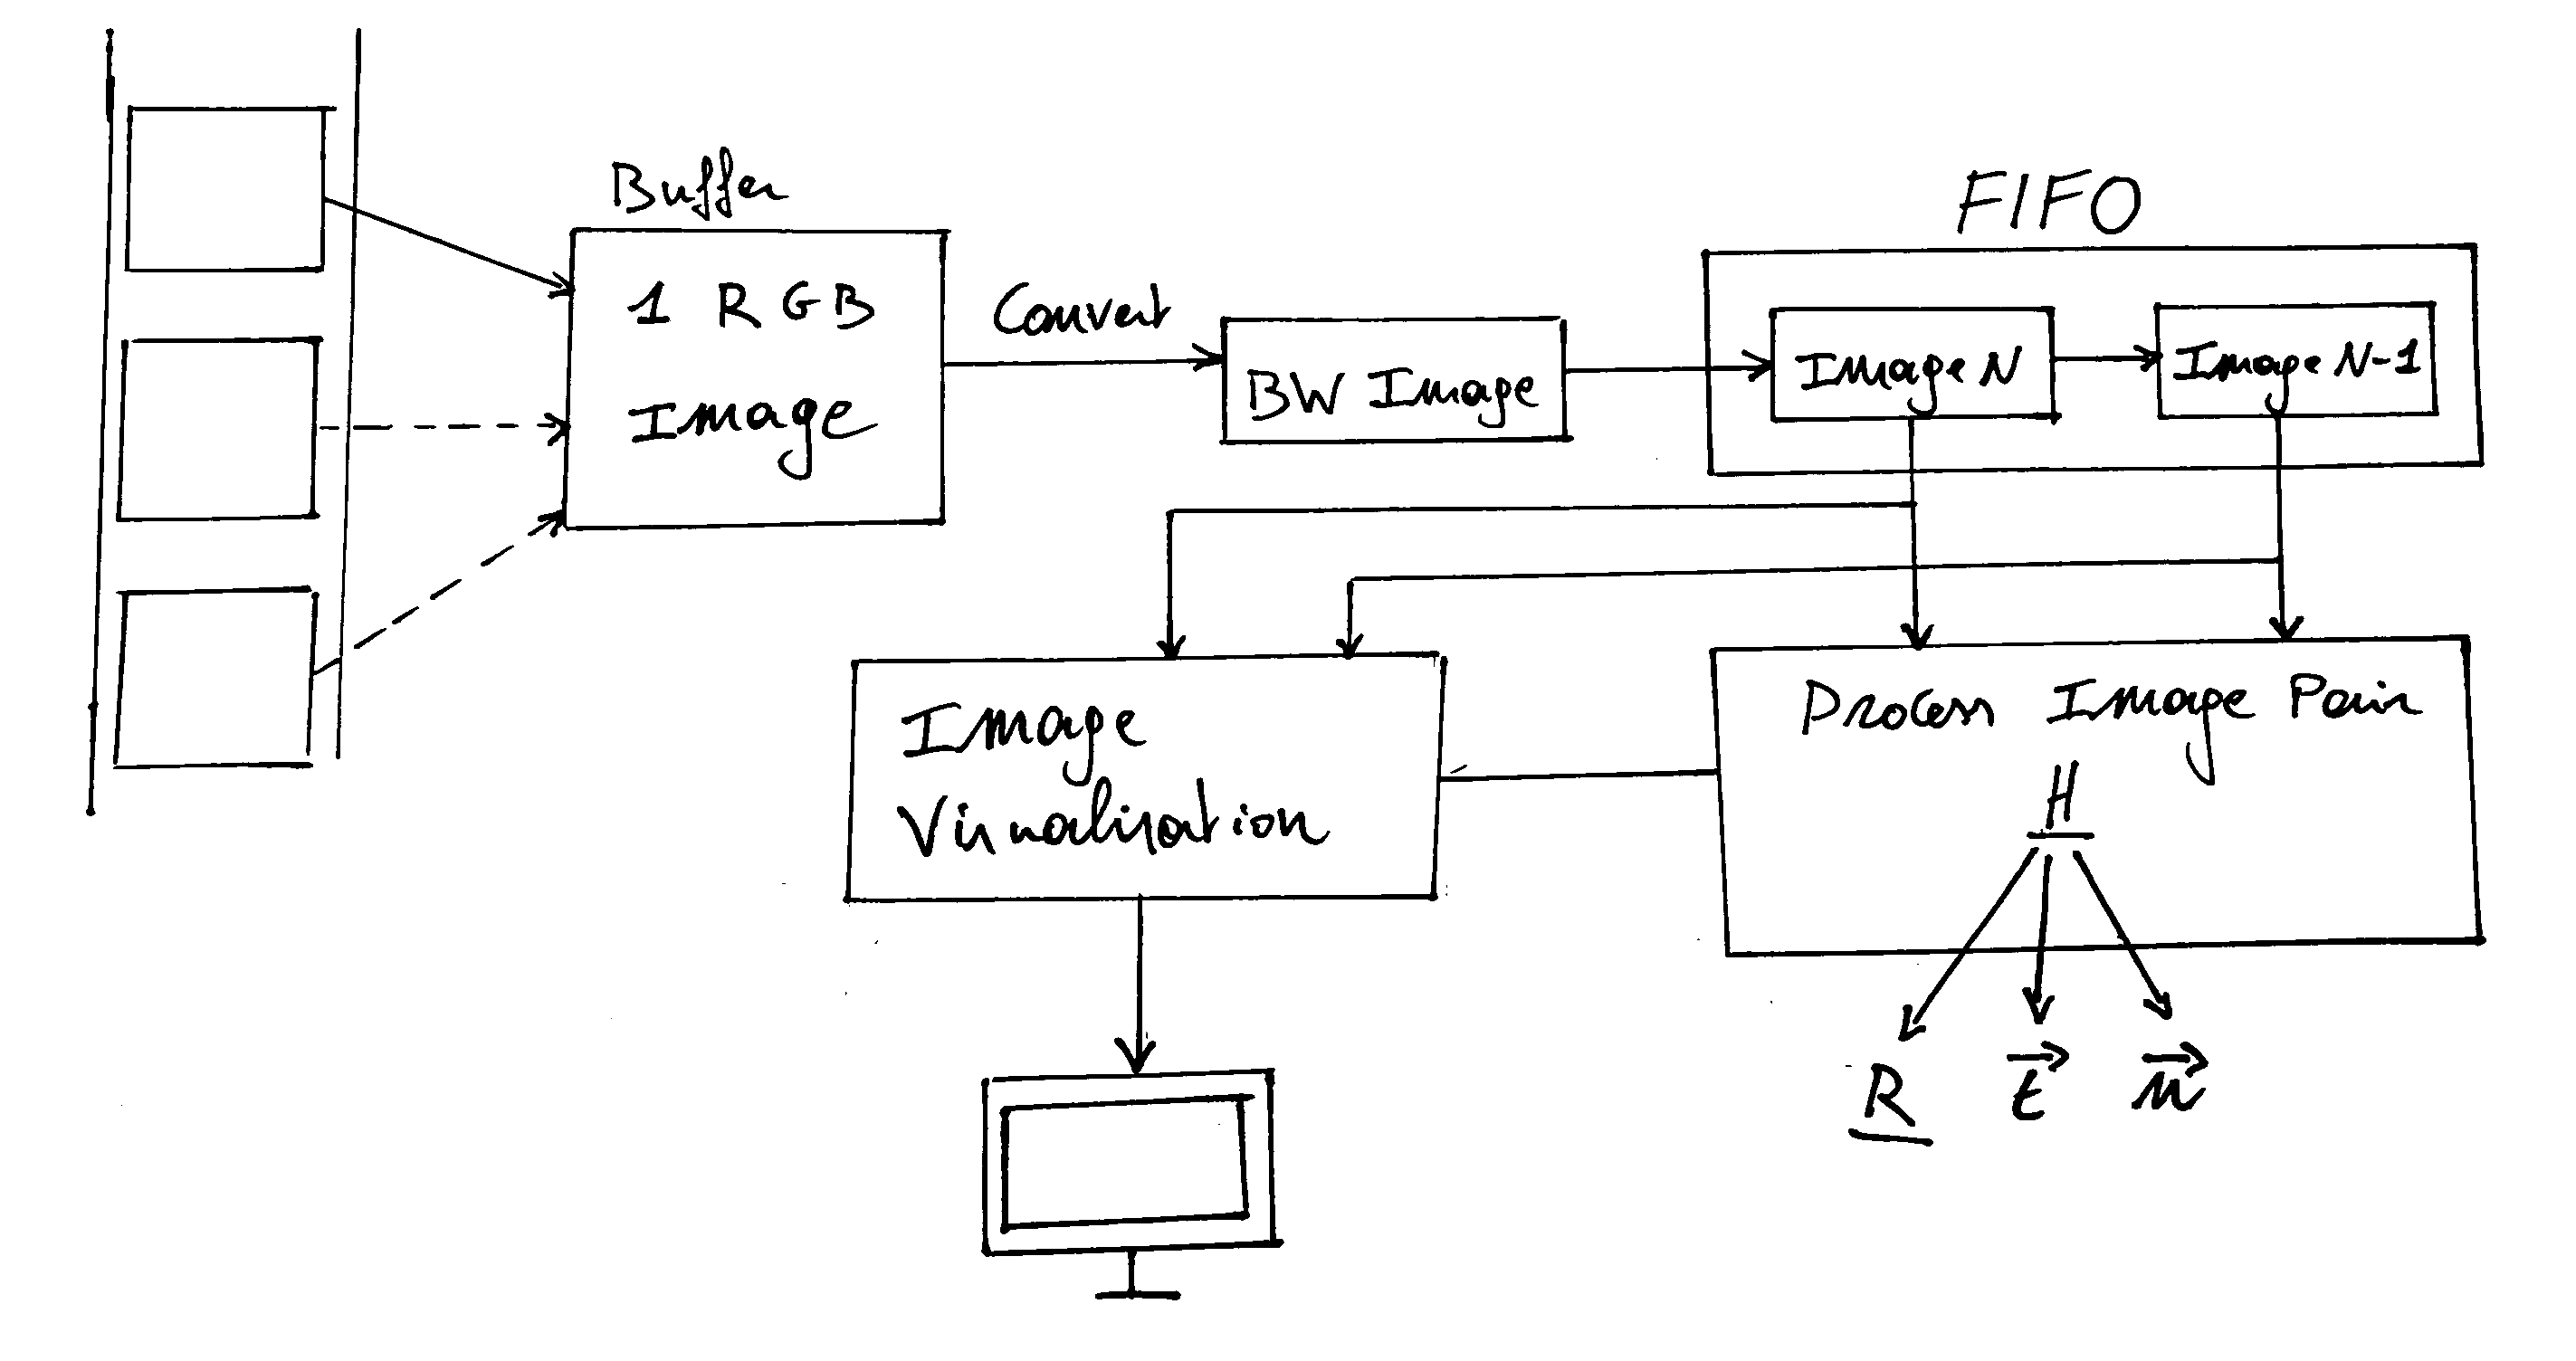
\includegraphics[width=1\textwidth]{figures/Block_diagram_sequencer.jpg}
    \caption{Scheme of sequencer}
    \label{fig:scheme}
\end{figure}

\section{Converting}
\subsection{Grayscale or color}
For now, the images are converted to grayscale. The big advantage is that a grayscale image only has one third of the information of an image in color with the same dimensions. Computationally everything will be faster using grayscale instead of color images. The drawback is a loss of information, but that drawback is rather small. The color of the image does not give us much more information to recognise structure and detect keypoints. So it is not worth the extra computations.\bigskip

However, in the footage we are using, the road is marked by colored cones. Most of the time the road is marked by yellow cones but sometimes there are blue cones on the road which means the car should slalom in between these cones. If at one point it should turn out the color of the cones is necessary, this will not be a problem. The newest image is always stored in the buffer in its original color, if we want to determine the color of the cone, this can easily be done by looking at the area where the cone is on the original image.

\subsection{Removing redundant information}\label{ssec:redundant}
As said before, the images are converted to grayscale. Next to that, they are also cropped. We are only interested in what is going on below the horizon, everything above it will not give us much information. In the footage we are using, there is not much to be cropped, because the footage we have is from a camera that was mounted tilted. Now that the sky and everything above the horizon is cropped out, there is one part of converting left.

\subsection{Masking out the ego-car}
\label{ssec:egocar}
The car itself is not moving relative to the camera, as the camera is fixed to the car, so it is irrelevant for the estimation of the movement. A mask is created to erase the car from the footage. This is only done when displaying the image however, otherwise the computation of keypoints would not work properly. When detecting the keypoints in the next step, keypoints laying in the area masked out by the ego-car, can be removed as keypoints. Figure \autoref{fig:input_image} shows an example of a frame before it is preprocessed. Figure \autoref{fig:output_image} shows the image after preprocessing. The black part is the masked out ego-car.

\begin{figure}
    \centering
    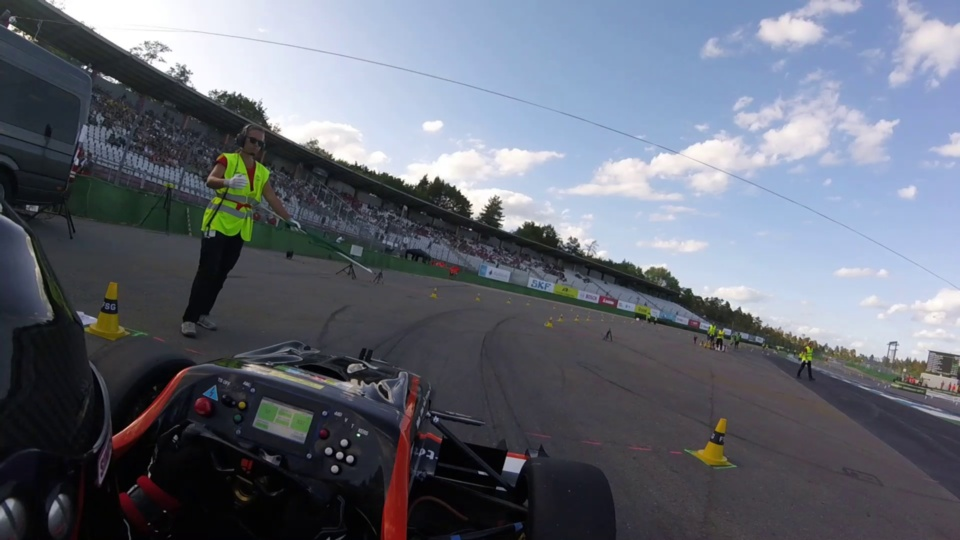
\includegraphics[width=1\textwidth]{figures/input_image.jpg}
    \caption{Input image}
    \label{fig:input_image}
\end{figure}

\begin{figure}
    \centering
    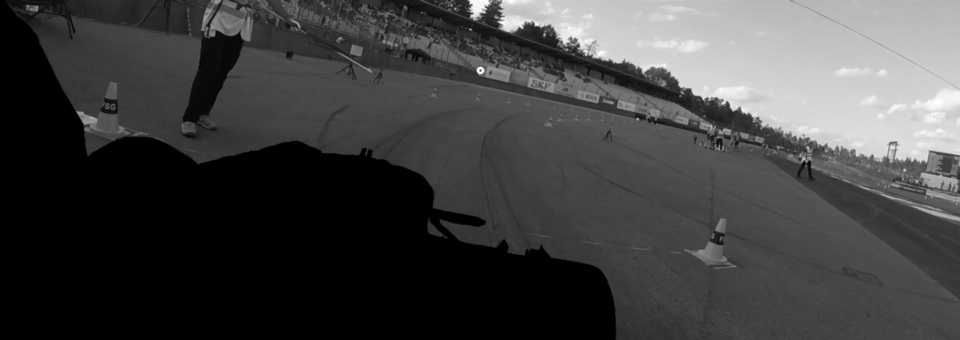
\includegraphics[width=1\textwidth]{figures/output_image.jpg}
    \caption{Preprocessed image}
    \label{fig:output_image}
\end{figure}

\section{Frame-to-frame motion of the car}
We can now step through the footage efficiently. To estimate the frame-to-frame motion of the car, the rotation matrix \underline{${R}$}, translation vector $\vec{t}$ and normal vector $\vec{n}$ must be calculated. These can be calculated using keypoints in the frames. 

\subsection{What are keypoints}
Keypoints are points in an image that carry a lot of information. If you were to take the point out of the image, it would be easy to recognise where the point is located in the image. To illustrate this, look at figure \autoref{fig:features}, this shows an image with 3 sections cut out. If you had to search for the place section C was cut out, it would be impossible as it could be almost anywhere. Section B is easier to locate, but you could move the cut horizontally without affecting the cut. Moving it vertically (along the gradient) the cut would change. Section A is the easiest to locate. There is no doubt as to where the cut is taken. Moving in either horizontal and vertical direction affects the cut.\bigskip

\begin{figure}
    \centering
    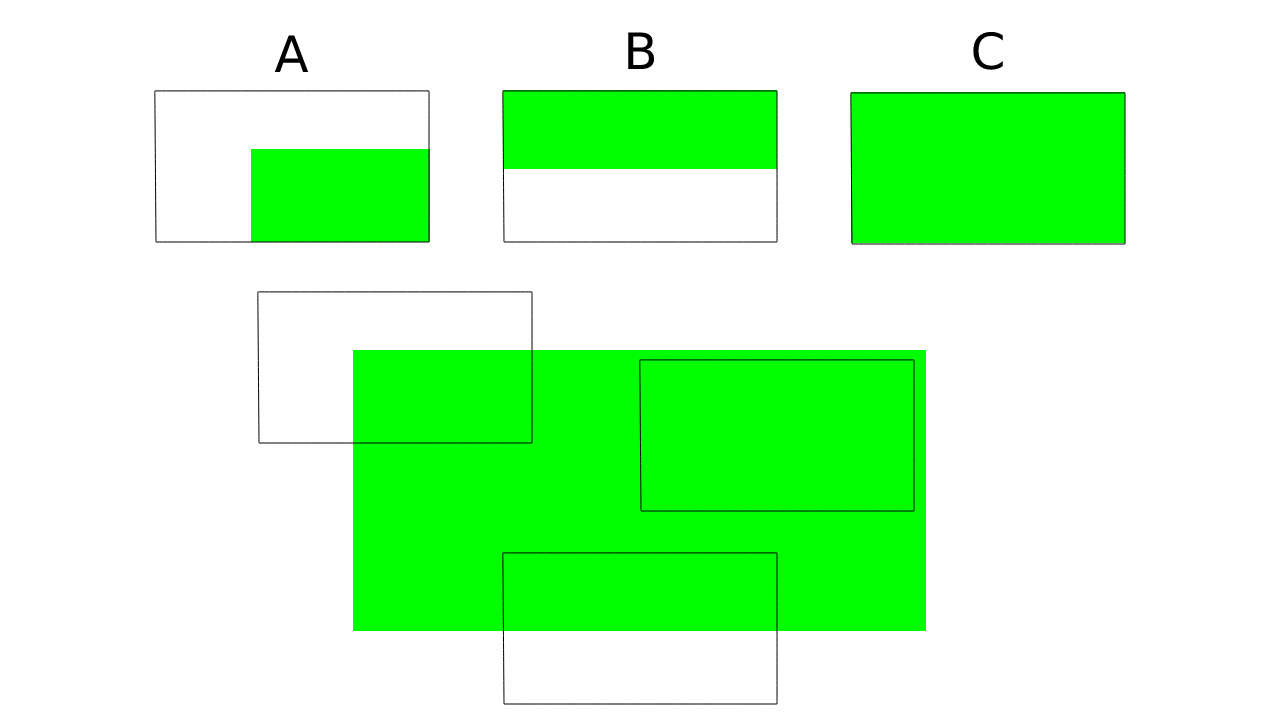
\includegraphics[width=1\textwidth]{figures/features.png}
    \caption{Keypoints in an image}
    \label{fig:features}
\end{figure}

This shows that corners are good keypoints in images as they have multiple gradients in different directions and can thus be easily located. Blobs could also be good keypoints. Blobs are a number of pixels that are connected through a common property.

\subsection{Matching keypoints}
The point in finding the keypoints is to know where these specific points are in another image. To match these keypoints, the region around the keypoint is looked at. This is called keypoint description and based on the description, matches are made between keypoints in different images. These matches hold the information to calculate the motion of the car.\bigskip

There are a lot of different methods and algorithms to find keypoints, describe them and match them.\bigskip

One way to match the keypoints is a Brute-Force Matcher. It is a rather simple matcher that takes the descriptor of a feature in image 1 and matches this descriptor with all the descriptors of image 2. It calculates the distance between these descriptors and returns the closest match. Different distance measurement types can be used. Cross checking is also a possibility, this means that matches are checked both ways. The matcher only returns those matches that are closest in both directions.

\subsection{ORB}
ORB or Oriented FAST and Rotated BRIEF is, as the name suggests, a combination of the FAST detector and BRIEF descriptor. ORB enhances the performance of the two with modifications. FAST is used to find keypoints, after which Harris Corner measure is used to find the top points among them. A pyramid scheme is used to produce multiscale-features. \bigskip 

One of the main advantages of ORB is the speed, according to Rublee et al. (2011) \cite{6126544} at two orders of magnitude faster than SIFT due to the fact that ORB is computationally more efficient. It is also more noise invariant and because of the speed useful in real-time applications.

\subsection{Filtering keypoints}
In \autoref{ssec:egocar} we already talked about the fact that keypoints part of the ego-car are considered noise as they are no part of the planar surface. But the keypoints are not the only keypoints that should be discarded. Everything above the horizon is not part of the planar surface either. In the future, we could try to detect the horizon and discard all keypoints above it, but for now we will do this manually.

As stated before, the footage we have is from a camera that is mounted tilted. This means we are not able to simply discard all keypoints above a horizontal line. We describe the horizon as a linear equation of the form
\begin{equation}\label{eq:linear}
    ax + by + c = 0
\end{equation}
To find the values for $a$, $b$ and $c$ we need two points on the horizon $p_1 = (x_1, y_1)$ and $ p_2 = (x_2, y_2)$. \autoref{eq:linear} can then be rewritten in terms of $p_1$ and $p_2$ as follows:
\begin{equation}
    (y_1-y_2)x + (x_2-x_1)y + (x_1y_2-x_2y_1) = 0
\end{equation}
For now an estimation suffices so we chose two points empirically. In \autoref{ssec:redundant} we already chose a height to cut off redundant information, this height was chosen based on the horizon. For $p_1$ we take this height as $y_1$ and as the camera is tilted to the right this is the leftmost point and $x_1 = 0$. For $p_2$ we chose a point at the utmost right of the image so $x_2$ is equal to the width of the image. For $y_2$ we choose a value by simply looking what seems to be the best option. \bigskip

\autoref{fig:key_orig} shows all keypoints detected without filtering out those above the horizon (keypoints on ego-car are already left out). \autoref{fig:key_filtered} shows what keypoints remain after filtering out those above the horizon. In both images, the horizon line is plotted to illustrate where our horizon lays.

\begin{figure}
    \centering
    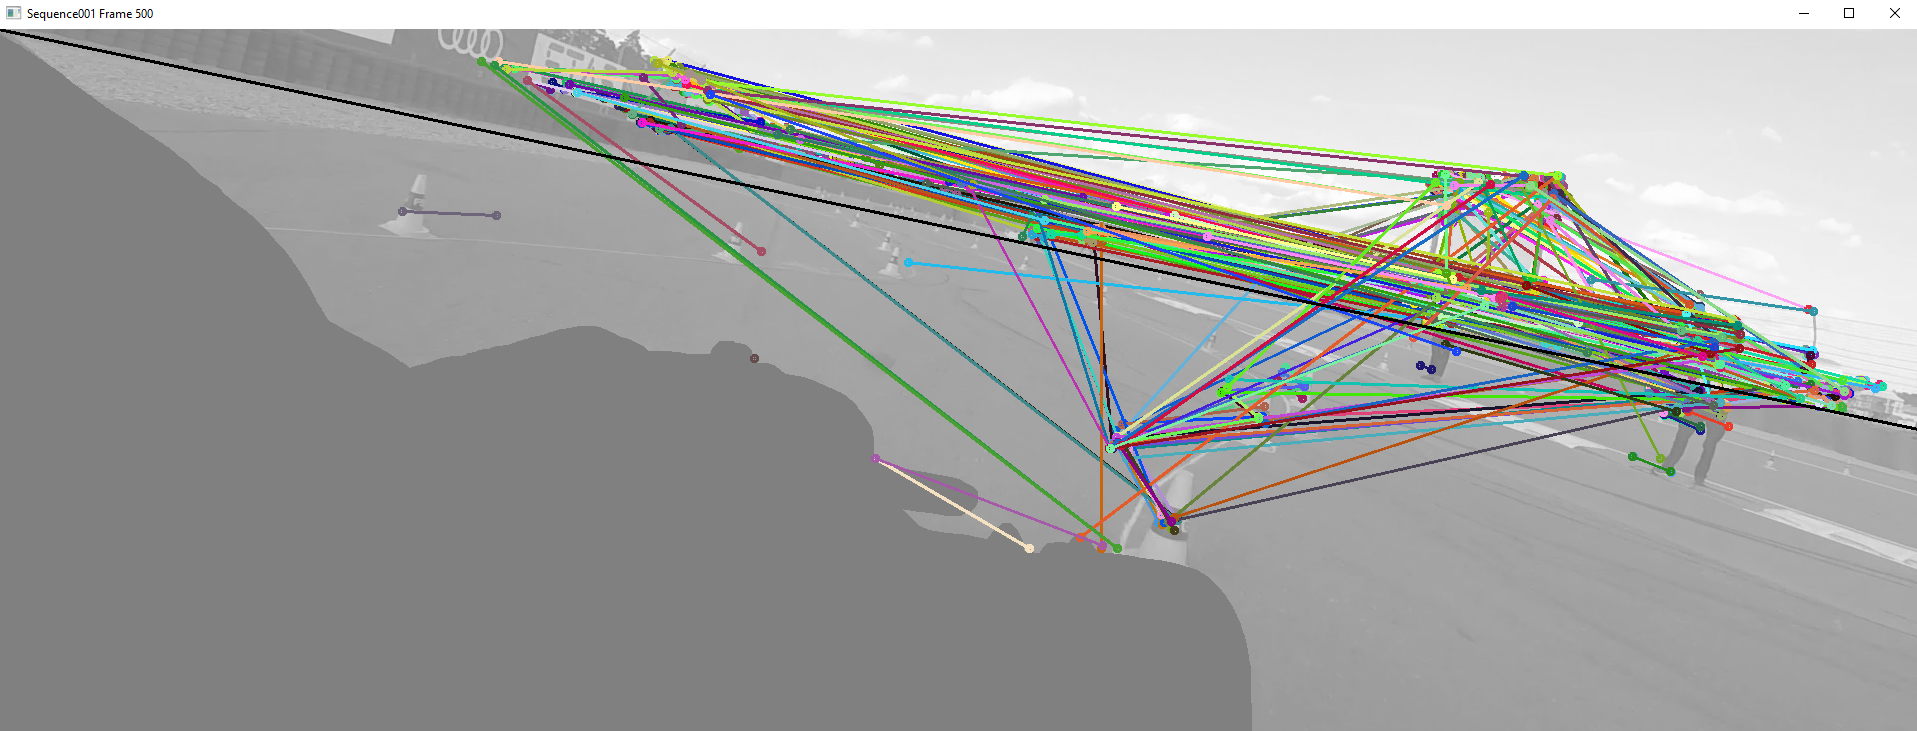
\includegraphics[width=1\textwidth]{figures/keypoint_orig.png}
    \caption{Keypoints before filtering}
    \label{fig:key_orig}
\end{figure}
\begin{figure}
    \centering
    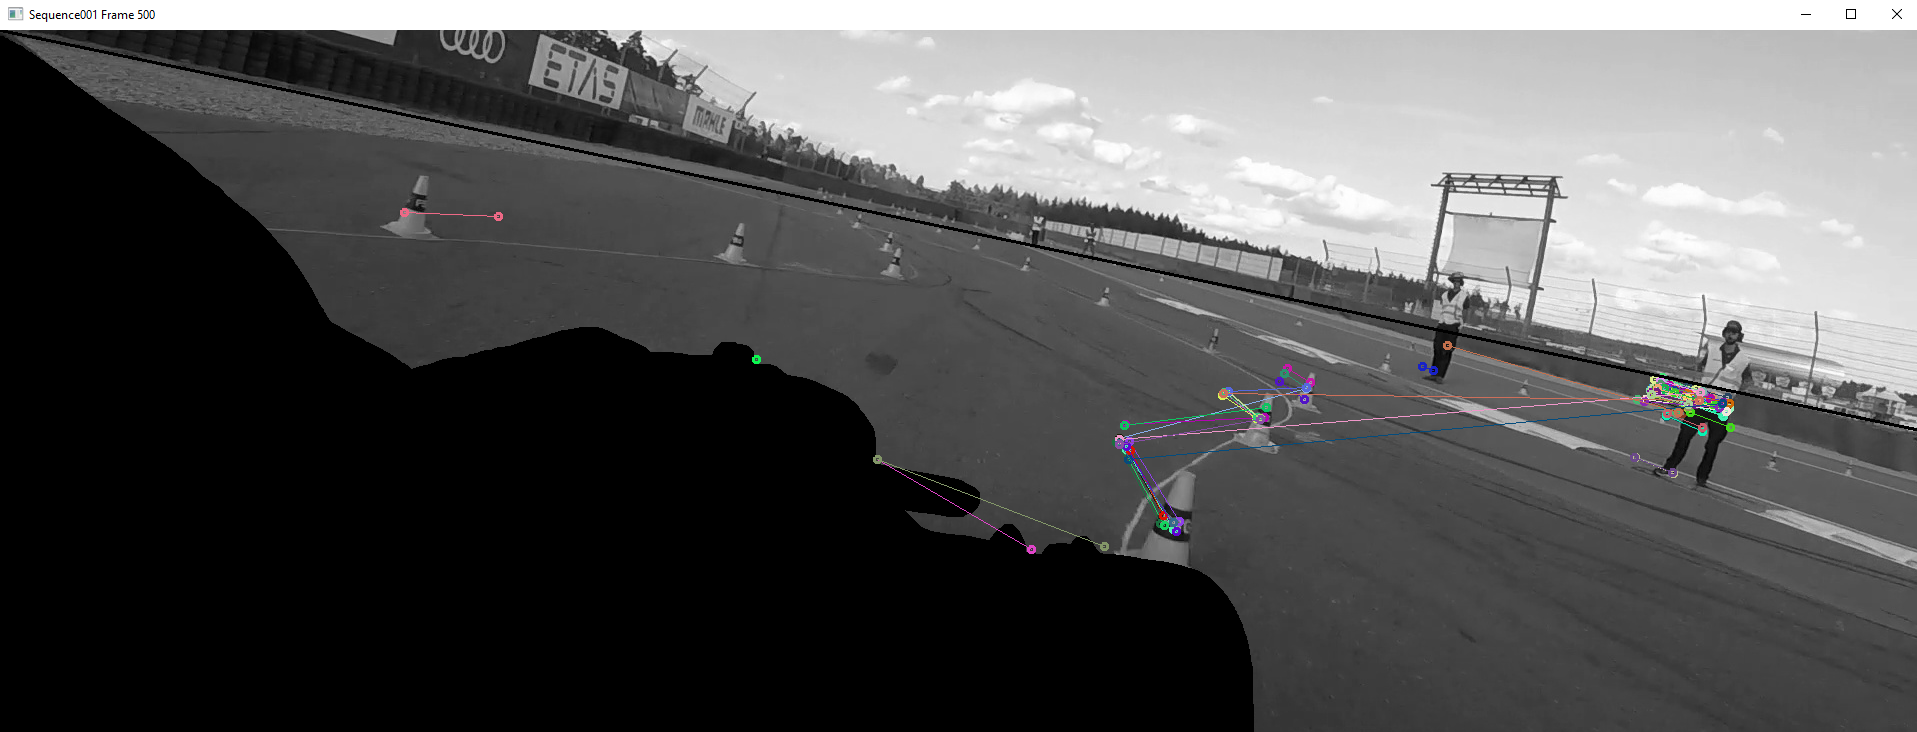
\includegraphics[width=1\textwidth]{figures/keypoint_filtered.png}
    \caption{Keypoints after filtering keypoints above the horizon}
    \label{fig:key_filtered}
\end{figure}